\documentclass[a4paper,french]{article}
\usepackage{authblk}
\usepackage{graphicx}

% for code colouring
\usepackage{pgf,pgfarrows,pgfnodes,pgfautomata,pgfheaps,pgfshade}
\usepackage{amsmath,amssymb}
\usepackage[latin1]{inputenc}
\usepackage{colortbl}
%%\usepackage[procnames]{listings}

% for code colouring
\usepackage{minted}
%%%%%%%%%%%%%%%%%%%%%

\usepackage{subfig}

\usepackage[frenchb]{babel}

\title{Introduction \`a \texttt{Go}\\ \&\\ Retours d'exp\'eriences}
\author{S\'ebastien Binet}
\date{Juin 2016}
\affil{CNRS/IN2P3/LPC}

\begin{document}
\maketitle

\section{Introduction}

Il n'y a plus de \emph{"Free Lunch"} possible: la loi de Moore~\cite{ref-moore}
n'est plus aussi ais\'ee \`a mettre en {\oe}uvre que par le pass\'e.
Les d\'eveloppeurs de logiciels, ainsi que les scientifiques, doivent maintenant
se familiariser avec la loi d'Amdahl~\cite{ref-amdahl}.
En effet, la fr\'equence d'horloge des processeurs n'augmente plus avec chaque
nouvelle g\'en\'eration: les processeurs gagnent de plus en plus de c\oe urs,
mais sans changer la fr\'equence par rapport \`a la g\'enr\'eration
pr\'ecedente.

L'augmentation du nombre de c\oe urs appelle \`a une utilisation plus
r\'epandue du parall\'elisme dans les logiciels d\'evelopp\'es par les
communaut\'es \texttt{HEP} et \texttt{Astro}.
Traditionnellement, le parall\'elisme a \'et\'e exploit\'e au niveau du
traitement des \'ev\'enements dans les logiciels de reconstruction et de
simulation des exp\'eriences de physique des particules: il suffit de lancer $N$
\emph{jobs} sur les fermes de calcul, la Grille ou un \emph{cloud}.
Plusieurs \'ev\'enements peuvent \^etre trait\'es en parall\`ele, m\^eme si les
algorithmes de reconstruction sont toujours appliqu\'es de mani\`ere
s\'equentielle \`a chacun de ces \'ev\'enements.

Cependant, chaque n\oe ud de calcul h\'ebergeant chacun de ces programmes, met \`a
disposition des ressources finies (empreinte m\'emoire, \emph{CPU}, descripteurs
de fichiers, \emph{sockets}, \emph{E/S}, etc\ldots), ressources dont le passage \`a
l'\'echelle est plus ardu lorsque l'empreinte m\'emoire des \emph{jobs} de
reconstruction des exp\'eriences du LHC atteint 2-4 $Gb$ de \texttt{RAM}.
Cette exploitation du parall\'elisme atteint ses limites avec les
ordres de grandeurs du LHC.

Ainsi, il semble plus efficace d'effectuer le traitement parall\`ele des
\'ev\'enements dans le m\^eme espace m\'emoire.
Pour un programme \'ecrit en \texttt{C++}, cela se traduit par l'utilisation de
plusieurs \emph{threads}.
Malheureusement, la programmation parall\`ele multi-t\^ache
(\emph{multithreading}) est notoirement connue pour ses difficult\'es de mise en
\oe uvre:
\begin{itemize}
	\item il est tr\`es ardu d'\'ecrire correctement une application \emph{multithread\'ee},
	\item il est \'egalement difficile de la garder correcte en fonction du
		temps,
	\item et aussi ardu de la garder efficace et optimis\'ee au cours des
		d\'eveloppements successifs.
\end{itemize}

De plus, m\^eme si \texttt{C++11}~\cite{ref-cxx11} et
\texttt{C++14}~\cite{ref-cxx14} apportent enfin la standardisation tant attendue
des APIs de programmation parall\`ele (\texttt{std::thread},
\texttt{std::mutex}, \texttt{std::future}), cela se fait au prix d'une
complexification encore plus pouss\'ee de ce langage, sans toutefois exposer une
API de haut niveau.
Il semble donc judicieux de se demander s'il n'existerait pas un nouveau langage
de programmation mieux adapt\'e \`a l'exploitation des architectures
parall\`eles\ldots

Pourquoi pas \texttt{Go}~\cite{ref-golang}?

\section{Anatomie de \texttt{Go}}

\texttt{Go} est un langage de programmation, libre (licence \texttt{BSD-3}),
initialement d\'evelopp\'e par Google et annonc\'e au monde en novembre 2009.
C'est un langage compil\'e, avec gestion automatique de la m\'emoire \emph{via} un
ramasse-miettes (\emph{garbage collector}), le support de la r\'eflection de
type, des fonctions anonymes, des \emph{closures} et de la programmation
orient\'ee objet.
La syntaxe de \texttt{Go} est r\'eminiscente du \texttt{C}.
Un bref aper\c cu d'un premier programme en \texttt{Go} est donn\'e dans la
figure~\ref{fig-go-hello}.

\begin{figure}[h]
\begin{minted}[linenos,frame=single,tabsize=4]{go}
// Command hello provides a greeting in french.
package main

import (
	"fmt"
)

func main() {
	fmt.Println("Bonjour la Lettre IN2P3.")
}
\end{minted}
\caption{\label{fig-go-hello}Un premier programme en \texttt{Go}.}
\end{figure}

\texttt{Go} est appr\'eci\'e pour sa capacit\'e \`a apporter au d\'eveloppeur
ainsi qu'\`a l'utili\-sa\-teur final, le meilleur des mondes "dynamique" et
"statique":
\begin{itemize}
	\item l'aisance de programmation des langages dynamiques gr\^ace \`a sa
		verbosit\'e limit\'ee, son syst\`eme d'inf\'erence de type et un cycle
		de d\'eveloppement \texttt{edit-compile-run} extr\^emement rapide,
	\item la robustesse d'un syst\`eme de typage statique,
	\item la vitesse d'un ex\'ecutable compil\'e en langage machine.
\end{itemize}

De plus, le support de \texttt{Go} pour les interfaces ressemble fortement au
\emph{duck-typing} de \texttt{Python}~\cite{ref-python} et se pr\^ete tr\`es
bien \`a l'\'ecriture de larges cadriciels (\emph{frameworks}) tels que ceux
utilis\'es et d\'evelopp\'es pour les exp\'eriences au LHC.

Enfin, \texttt{Go} expose un support accru et int\'egr\'e au langage, de la
programmation concurrente \emph{via} le mod\`ele \emph{CSP} (\emph{Communicating
Sequential Processes}~\cite{ref-csp}).
En effet, il suffit de pr\'efixer l'appel \`a une m\'ethode avec le mot-cl\'e
\texttt{go} pour que son ex\'ecution s'effectue de mani\`ere concurrente aux
autres fonctions, et ce, dans un \emph{thread} l\'eger appel\'e
\texttt{goroutine}.
Les \texttt{goroutines} sont multiplex\'ees sur plusieurs \emph{threads} natifs:
une \texttt{goroutine} bloqu\'ee, par exemple, par une op\'eration d'\texttt{E/S}
(disque, r\'eseau, etc\ldots), n'emp\^echera pas l'ex\'ecution des autres
\texttt{goroutines} du programme.
De plus, les \texttt{goroutines} sont tr\`es peu gourmandes en ressources
gr\^ace \`a leur pile de petite taille et ajust\'ee \`a l'ex\'ecution.
Ceci permet d'en lancer un tr\`es grand nombre et ce sur des machines modestes:
il n'est pas rare de voir des programmes comportant des milliers de
\texttt{goroutines} sur des laptops aux capacit\'es modestes, prouesse
impossible avec des \emph{threads} natifs.

Dans le langage \texttt{Go}, le m\'ecanisme permettant d'\'echanger des
donn\'ees entre \texttt{goroutines} et ce sans circonvenir la s\^uret\'e du
syst\`eme de typage (\emph{type safety}), est appel\'e un \texttt{channel}.
Envoyer et recevoir des donn\'ees par un \texttt{channel} sont des op\'erations
atomiques et permettent donc de synchroniser l'ex\'ecution des
\texttt{goroutines}.
Un exemple de communication entre \texttt{goroutines} est donn\'e dans la
figure~\ref{fig-goroutine}: la \texttt{goroutine} principale, \texttt{main},
lance deux \texttt{goroutines}, \texttt{gen} et \texttt{square}.
\texttt{gen} g\'en\`ere la suite des nombres entiers de $0$ \`a $+\infty$ et
remplit le \texttt{channel} \texttt{in}.
\texttt{square} extrait les nombres entiers de ce \texttt{channel} et remplit le
\texttt{channel} \texttt{out} avec le carr\'e de ces nombres.
La \texttt{goroutine} \texttt{main} extrait les donn\'ees du \texttt{channel}
\texttt{out} et les affiche \`a l'\'ecran.

\begin{figure}[h]
\begin{minted}[linenos,frame=single,tabsize=4]{go}
package main

func main() {
	in := make(chan int)
	out := make(chan int)
	go gen(in)
	go square(out, in)
	for i := range out {
		println(i)
	}
}

// gen generates numbers [0...)
func gen(ch chan int) {
	i := -1
	for {
		i++
		ch <- i
	}
}

// square returns the square of each number.
func square(out, in chan int) {
	for i := range in {
		out <- i*i
	}
}
\end{minted}
	\caption{\label{fig-goroutine}Deux \texttt{goroutines}, \texttt{gen} et
	\texttt{square} se communiquent des donn\'ees.}
\end{figure}

\texttt{Go} permet \'egalement d'appeler ais\'ement du \texttt{C} \emph{via}
\texttt{cgo}~\cite{ref-cgo}.
Il suffit d'importer le pseudo \texttt{package} \texttt{"C"} et d'indiquer les
fichiers d'en-t\^ete et biblioth\`eques pour utiliser les fonctions et types
expos\'es par cette biblioth\`eque \texttt{C}.
Un exemple est donn\'e dans la figure~\ref{fig-cgo}.

\begin{figure}[h]
\begin{minted}[linenos,frame=single,tabsize=4]{go}
package main

// #cgo LDFLAGS: -lm
// #include <math.h>
import "C"

func main() {
	println("C.sqrt(4)=", C.sqrt(4))
}
\end{minted}
	\caption{\label{fig-cgo}Programme \texttt{Go} utilisant la fonction
	\texttt{sqrt} de la biblioth\`eque \texttt{C} \texttt{libm}.}
\end{figure}

Depuis la publication de la version \texttt{1.0} de \texttt{Go} en 2012, le
langage est consid\'er\'e stable et compl\'etement r\'etro-compatible: chaque
nouvelle version de \texttt{Go} (une tous les six mois en moyenne) compilera
correctement un programme valide de 2012.
Ce contrat de stabilit\'e est \'egalement appliqu\'e \`a la biblioth\`eque
standard livr\'ee avec le compilateur.

De part son origine et son ADN, \texttt{Go} permet de d\'evelopper rapidement de
larges programmes.
Son mod\`ele de compilation d'\'executables statiques permet \'egalement de les
d\'eployer ais\'ement sur de larges infrastructures: \texttt{Go} est rapidement
devenu la \emph{lingua franca} du d\'eveloppement \emph{cloud}.
Est-il adapt\'e \`a l'environnement HEP et astro?

\section{Retours d'exp\'eriences}

%% fads, fwk
%% go-lsst/fcs-ctl
%% go-lsst/snfusion

\subsection{Analyse \& simulation}

\texttt{Go} a d'abord fait ses d\'ebuts dans HEP \emph{via} la
r\'eimpl\'ementation du \emph{framework} de contr\^ole hors-ligne d'ATLAS et LHCb:
\textsc{Gaudi}~\cite{ref-gaudi}.
Cette r\'eimpl\'ementation, appel\'ee simplement \texttt{fwk}, est regroup\'ee
sous l'ombrelle de l'organisation \texttt{go-hep}~\cite{ref-gohep}.
Le but principal de \texttt{go-hep/fwk}~\cite{ref-gohep-fwk} \'etait de
d\'emontrer la viabilit\'e et l'ad\'equation de \texttt{Go} pour les
\emph{control frameworks} LHC, mais \'egalement de montrer l'aisance avec
laquelle la programmation parall\`ele peut \^etre mise en \oe uvre avec
\texttt{Go}.

Un autre axe de travail \'etait de montrer qu'un cadriciel concurrent comme
\texttt{fwk} \'etait non seulement adapt\'e aux grosses exp\'eriences LHC avec
leur infrastructure sous-jacente, mais \'etait \'egalement adapt\'e aux
entreprises de plus petites tailles telles qu'une analyse individuelle ou bien
une biblioth\`eque de simulation.
En effet, une des critiques r\'ecurrentes des physiciens vis-\`a-vis de
\textsc{Gaudi} est sa lourdeur d'impl\'ementation ainsi que la difficult\'e de
l'installer sur une machine de bureau, ce qui en fait une
plateforme de d\'eveloppement d'analyses peu s\'eduisante, malgr\'e sa
robustesse et sa capacit\'e \`a traiter les volumes de donn\'ees du LHC.

Cet axe de travail a \'et\'e concr\'etis\'e sous la forme de
\texttt{fads}~\cite{ref-fads}.
\texttt{fads} est la r\'eimpl\'ementation de
\textsc{Delphes}~\cite{ref-delphes}, un simulateur de d\'etecteur de physique
des particules.
\textsc{Delphes} est un ensemble de composants \texttt{C++} bas\'es sur
\textsc{Root} dont le \emph{design} ne se pr\^ete pas ais\'ement \`a une
impl\'ementation \emph{multithread\'ee}.
Les d\'etails de la comparaison entre les deux applications sont disponibles
dans~\cite{ref-fads-hsf}: le passage \`a l'\'echelle de \texttt{fads} est
nettement meilleur que \textsc{Delphes}, tant en empreinte m\'emoire qu'en
fr\'equence de traitement d'\'ev\'enements.
Ces performances sont report\'ees dans la figure~\ref{fig-fads-delphes}.

Au cours du d\'eveloppement de \texttt{fads}, plusieurs biblioth\`eques
d'interfa\c cage avec l'existant (\textsc{Root}, \texttt{HepMC},
\texttt{HEPEVT}) ont du \^etre d\'evelopp\'ees, ainsi que des biblioth\`eques
d'analyse (histogrammes, \emph{plot}s).
Ce travail a permis de montrer que \texttt{Go} est un langage viable et
comp\'etitif dans le cadre du calcul et de l'analyse de donn\'ees, et ce, m\^eme
dans le microcosme HEP.

\begin{figure}[h]
	\begin{center}
	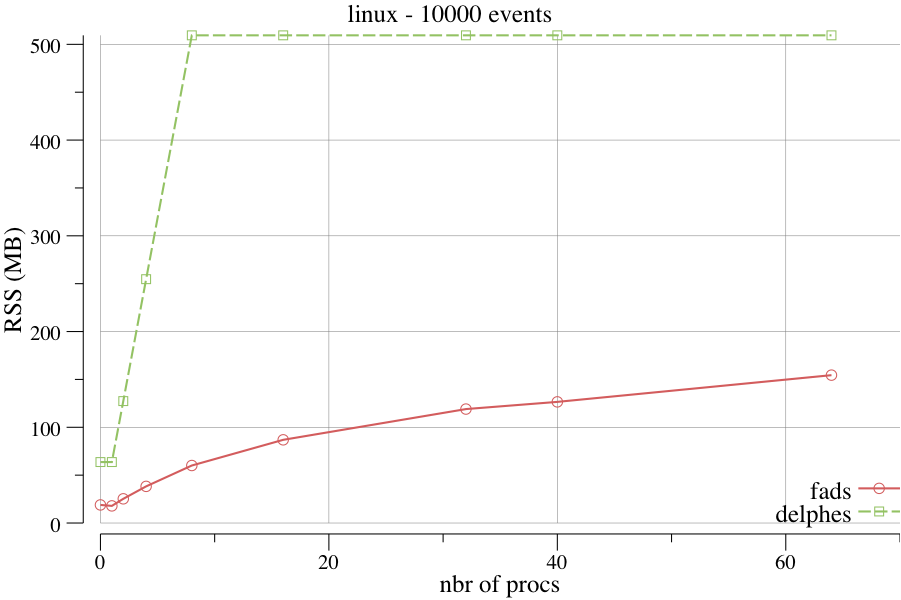
\includegraphics[width=14pc]{figs/lhcb3-rss.png}
	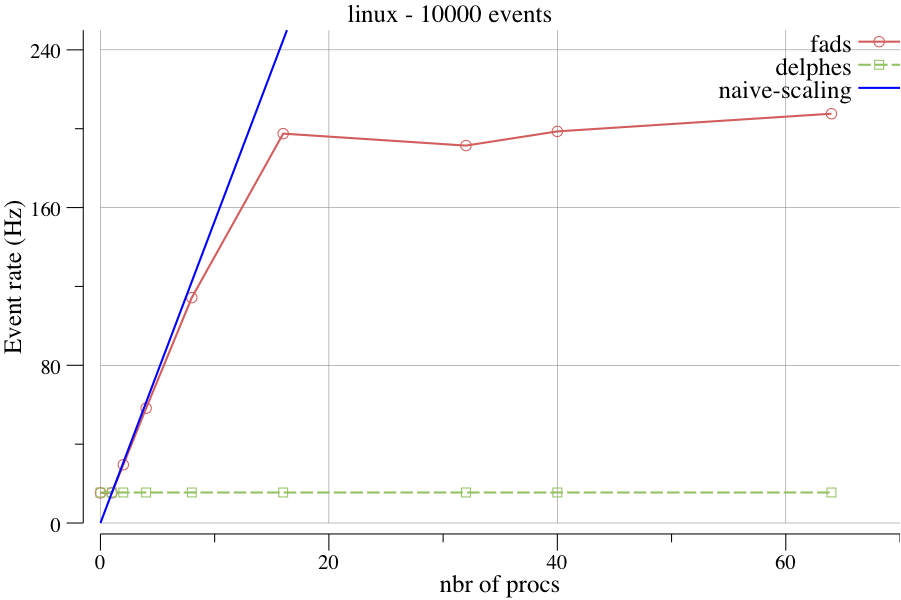
\includegraphics[width=14pc]{figs/lhcb3-hz.png}
	\end{center}
	\caption{\label{fig-fads-delphes}Empreinte m\'emoire (\`a gauche) et
	fr\'equence de traitement des \'ev\'enements (\`a droite). R\'esultats
	obtenus sur un serveur \texttt{Linux} de 40 c\oe urs (20 physiques).
	\`A noter que, pass\'es 8 processus concurrents, le serveur n'avait plus
	assez de ressources (RAM) pour \textsc{Delphes}.}
\end{figure}

\subsection{Contr\^ole commande \& monitoring}

Un axe de recherche plus r\'ecent est l'investigation de \texttt{Go} et sa
pertinence dans le monde du contr\^ole commande.
Dans le cadre de l'exp\'erience LSST, un banc de test pour la caract\'erisation
des moteurs pour le changeur de filtres de la cam\'era devait \^etre
r\'ealis\'e.
Ces moteurs peuvent \^etre command\'es \emph{via} plusieurs interfaces et
protocoles (\textsc{CANBus}, \textsc{ModBus}, \ldots): c'est le protocole
\textsc{ModBus} qui a \'et\'e finalement retenu et mis en \oe uvre.

Malgr\'e la jeunesse de \texttt{Go}, une biblioth\`eque prenant en charge le
protocole \textsc{ModBus} \'etait d\'ej\`a disponible sous licence libre,
distribu\'ee \emph{via} \texttt{github}~\cite{ref-go-modbus} et \'ecrite par la
communaut\'e.
Comme pour tous les \texttt{packages} \texttt{Go}, une simple commande a suffi
pour installer cette biblioth\`eque:

\begin{center}
\begin{verbatim}
$> go get github.com/goburrow/modbus
\end{verbatim}
\end{center}

L'application permettant d'envoyer des commandes aux moteurs, de
\emph{monitorer} leurs positions, temp\'eratures et autres grandeurs est en fait
un serveur web \'ecrit en \texttt{Go}.
En effet, l'offre des GUIs en \texttt{Go} est encore limit\'ee: m\^eme s'il
existe des \emph{bindings} vers la plupart des biblioth\`eques graphiques
portables (Qt, GTK, \ldots), leur installation n'est pas aussi ais\'ee qu'un
\texttt{package} \'ecrit totalement en \texttt{Go}.
Il existe bien le d\'ebut d'une biblioth\`eque en \texttt{Go}, mais elle est
encore en chantier~\cite{ref-go-shiny}.
La solution retenue a donc \'et\'e l'\'ecriture d'un ex\'ecutable servant une
page web HTML5 utilisant \texttt{Polymer}~\cite{ref-polymer} pour r\'ealiser
l'interface graphique.
L'utilisateur envoie des commandes depuis l'interface, commandes qui sont
ensuite relay\'ee au serveur \emph{via} des WebSockets.
Le serveur se charge de la communication avec les moteurs et renvoie
r\'esultats des commandes, histogrammes, flux vid\'eo et grandeurs
\emph{monitor\'ees} \`a l'utilisateur au moyen d'un autre WebSocket.
L'authentification des utilisateurs ainsi que la syndicalisation des flux et
connexions sont g\'er\'ees c\^ot\'e serveur.
Cette architecture orient\'ee web permet \emph{in fine} une grande transparence
r\'eseau, et ce, m\^eme pour des clients Windows.
La figure~\ref{fig-fcs-lsst} constitue un aper\c cu de l'interface graphique.

\begin{figure}[h]
	\begin{center}
	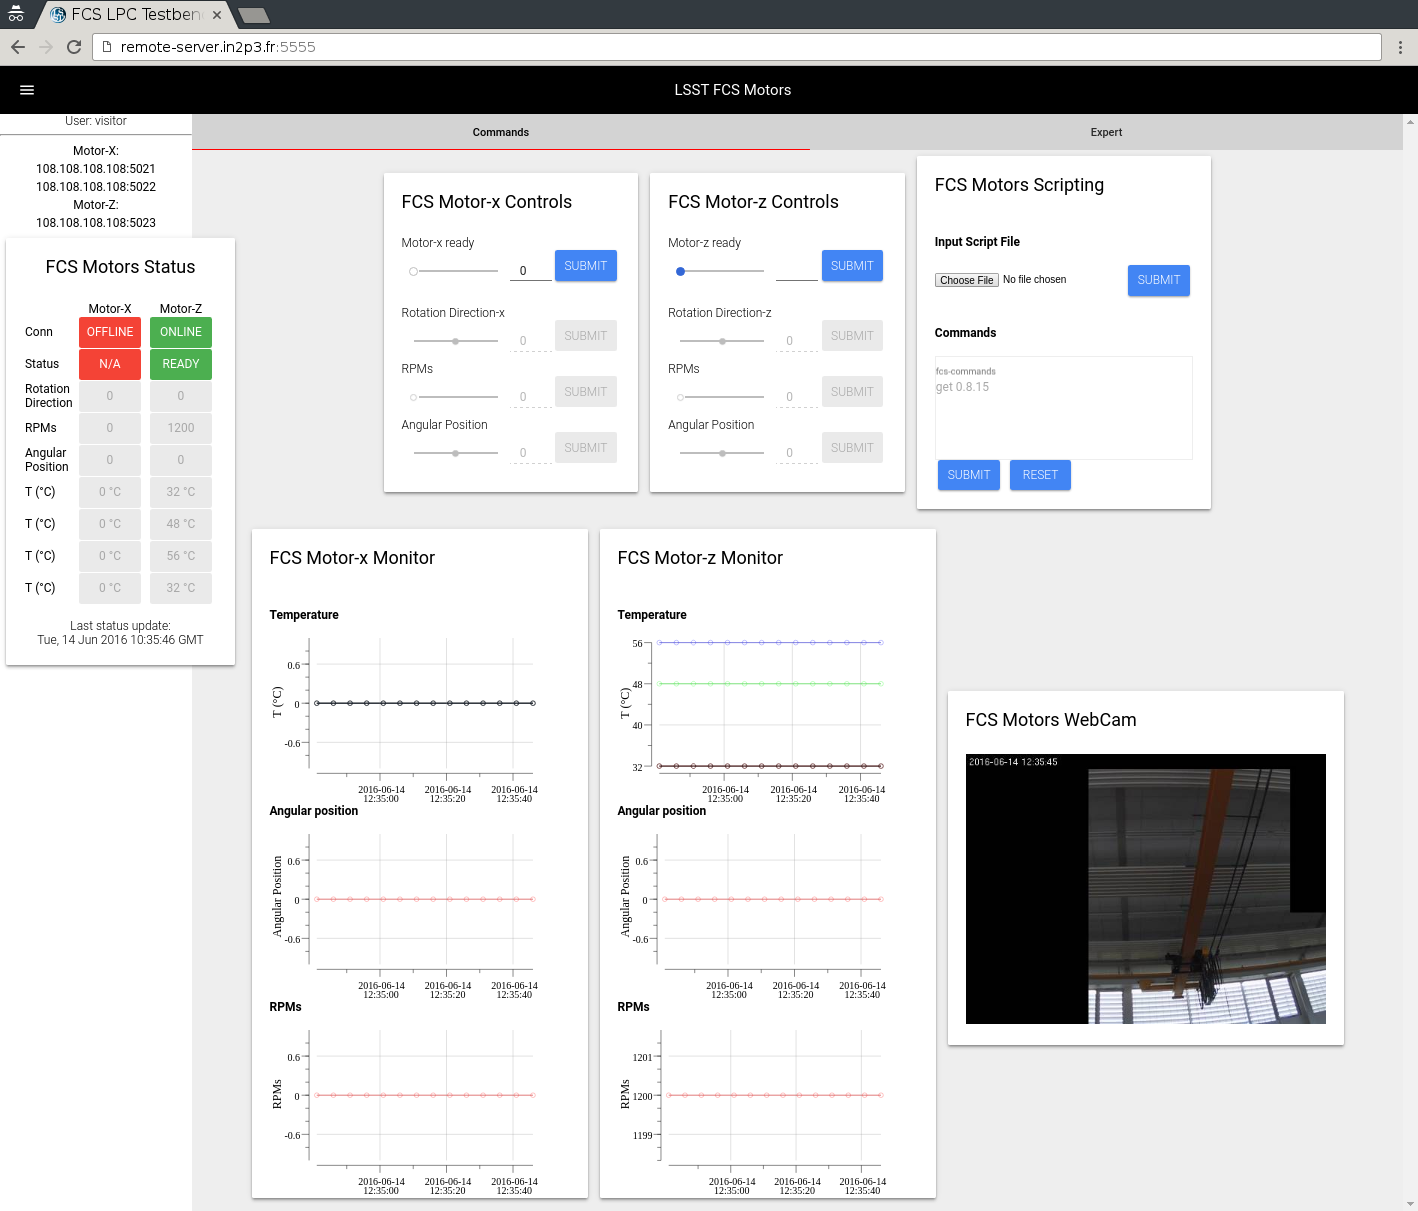
\includegraphics[width=20pc]{figs/fcs-lsst.png}
	\end{center}
	\caption{\label{fig-fcs-lsst}Interface graphique pour le banc de test du
	LPC. L'interface est en HTML5/\texttt{Polymer}, le serveur en \texttt{Go}.}
\end{figure}

\section{Conclusions}

Cet article a pr\'esent\'e le langage \texttt{Go}.
Son approche pragmatique et sa volont\'e de rester simple (mais pas simpliste),
coupl\'ees \`a son mod\`ele de programmation concurrente, font de \texttt{Go} un
langage r\'esolument adapt\'e \`a l'environnement plus h\'et\'erog\`ene des
machines multi-c\oe urs d'aujourd'hui et de demain.

Malgr\'e son relatif jeune \^age, \texttt{Go} comporte d\'ej\`a la plupart des
biblioth\`eques n\'ecessaires \`a la programmation d'applications de calcul et
d'analyse.
Les outils int\'egr\'es \`a la cha\^ine de d\'eveloppement de \texttt{Go}
permettent de plus de rapidement optimiser un code donn\'e (CPU, m\'emoire,
concurrence, I/O, \ldots).
Enfin, l'empreinte m\'emoire r\'eduite de \texttt{Go} par rapport \`a
\texttt{Java} et ses facilit\'es en programmation concurrente, en font une
alternative cr\'edible dans le domaine de l'acquisition et \emph{monitoring}
de donn\'ees, et le contr\^ole commande.

\texttt{Go} est d'ores et d\'ej\`a le langage du \emph{cloud}.
Peut-\^etre aura-t-il une vie dans HEP et en Astro?
Une chose est s\^ure: il a tous les atouts pour y arriver et supplanter
\texttt{C++}, \texttt{Python} et \texttt{Java}.

\begin{thebibliography}{9}
	\bibitem{ref-moore} Moore E, "Cramming more components onto integrated circuits",
		\\ Electronics Magazine, 1965
	
	\bibitem{ref-amdahl} Amdahl G, "Validity of the Single Processor Approach to Achieving Large-Scale Computing Capabilities", AFIPS Conference Proceedings, (30), pp. 483-485, 1967
	
	\bibitem{ref-cxx11} The \texttt{C++11} programming language, \\
		\verb'http://www.open-std.org/jtc1/sc22/wg21/docs/papers/2010/n3092.pdf'

	\bibitem{ref-cxx14} The \texttt{C++14} programming language, \\
		\verb'http://www.open-std.org/jtc1/sc22/wg21/docs/papers/2013/n3797.pdf'

	\bibitem{ref-golang} \texttt{Go},
		\verb'https://golang.org'

	\bibitem{ref-python} The \texttt{Python} programming language,
		\verb'http://python.org'

	\bibitem{ref-csp} CSP,
		 \verb'http://en.wikipedia.org/wiki/Communicating_sequential_processes'

	\bibitem{ref-cgo} \texttt{cgo},
		\verb'https://golang.org/cmd/cgo/'

	\bibitem{ref-gaudi} Mato P 1998 \textsc{Gaudi}-architecture design document Tech.
		Rep.\\ LHCb-98-064 Geneva
	
	\bibitem{ref-gohep} The \texttt{go-hep} project,
		\verb'https://github.com/go-hep'


	\bibitem{ref-gohep-fwk} The \texttt{go-hep/fwk} concurrent control
		framework,\\
		\verb'https://github.com/go-hep/fwk'

	\bibitem{ref-fads} \texttt{fads}: a Fast Detector Simulation toolkit,\\
		\verb'https://github.com/go-hep/fads'

	\bibitem{ref-delphes} DELPHES 3: a modular framework for fast simulation of
		a generic collider experiment,
		\verb'arXiv:1307.6346'

	\bibitem{ref-fads-hsf} \texttt{fads} @ HEP Software Foundation workshop,\\
		\verb'https://indico.cern.ch/event/357737/contributions/1770401/'

	\bibitem{ref-go-modbus} \verb'https://github.com/goburrow/modbus'

	\bibitem{ref-go-shiny}
	\verb'https://github.com/golang/exp/tree/master/shiny'

	\bibitem{ref-polymer} \verb'https://www.polymer-project.org/'
	
\end{thebibliography}

\end{document}
